\documentclass[11pt]{article}

\usepackage[margin=1in]{geometry}
\usepackage{booktabs}
\usepackage{graphicx}
\usepackage{amsmath}
\usepackage{xeCJK}
\usepackage{hyperref}
\usepackage{microtype}

\setCJKmainfont{SimSun}
\setmainfont{Times New Roman}

\title{真实焦栈 Focus Confidence 诊断报告}
\author{SRTP Optical Mechanism Analysis}
\date{2026-06-22}

\begin{document}
\maketitle

\section{Research Question}

前两轮 synthetic 实验显示，DFF failure 更直接地对应 focus-response 置信度结构，尤其是 top-2 focus margin，而几何 glare risk 更适合作为物理解释先验。真实样本缺少逐像素高度真值，因此本轮不评估 absolute MAE，而是检查真实焦栈内部是否存在与该机制一致的无参考证据：高亮/过曝区域是否对应早层 focus peak，confidence maps 是否能定位 DFF peak layer 的局部跳变，以及 saturation persistence 与 focus confidence 是否对应不同类型的不可靠性。

\section{Method}

脚本读取 40 层真实焦栈，并统一缩放到 $512 \times 640$。使用 Laplacian focus measure 构造 DFF focus volume，并计算 DFF peak layer、\texttt{low\_margin}、\texttt{focus\_entropy}、\texttt{low\_peak\_strength}、\texttt{sat\_persistence}、\texttt{bright\_persistence}、\texttt{spike\_proxy} 和 \texttt{quality\_proxy}。

\texttt{spike\_proxy} 是 DFF peak layer 与局部邻域均值的偏离程度，用于描述层选择局部不稳定性。\texttt{sat\_persistence} 是焦栈中 $I \geq 0.98$ 的层数比例，用于描述强高亮或过曝持续性。二者都不是 ground-truth error，只能作为无参考诊断。

\section{ROI Results}

\begin{table}[htbp]
\centering
\small
\begin{tabular}{lrrrrrr}
\toprule
ROI & Peak layer & Low margin & Entropy & Sat. persist. & Spike proxy & Quality \\
\midrule
\texttt{highlight\_edge} & 3.03 & 0.7910 & 0.8454 & 0.0364 & 0.0204 & 0.5877 \\
\texttt{ordinary\_texture} & 18.88 & 0.8395 & 0.9757 & 0.0000 & 0.1174 & 0.6451 \\
\texttt{dark\_region} & 18.49 & 0.8442 & 0.9794 & 0.0000 & 0.1223 & 0.6506 \\
\bottomrule
\end{tabular}
\caption{ROI-level no-reference diagnostics on the real focus stack.}
\end{table}

\begin{table}[htbp]
\centering
\small
\begin{tabular}{lrrrr}
\toprule
Score & Spearman spike & AUC spike & AUC saturation & AUC early peak \\
\midrule
\texttt{low\_margin} & 0.4710 & 0.7293 & 0.5002 & 0.4420 \\
\texttt{focus\_entropy} & 0.6136 & 0.7804 & 0.4091 & 0.2048 \\
\texttt{low\_peak\_strength} & 0.7085 & 0.8491 & 0.4649 & 0.2090 \\
\texttt{sat\_persistence} & 0.1251 & 0.5384 & 1.0000 & 0.6728 \\
\texttt{bright\_persistence} & 0.0738 & 0.5172 & 0.9780 & 0.6792 \\
\texttt{quality\_proxy} & 0.6522 & 0.9289 & 0.5182 & 0.4367 \\
\bottomrule
\end{tabular}
\caption{Association between confidence scores and no-reference proxies.}
\end{table}

\begin{figure}[htbp]
\centering
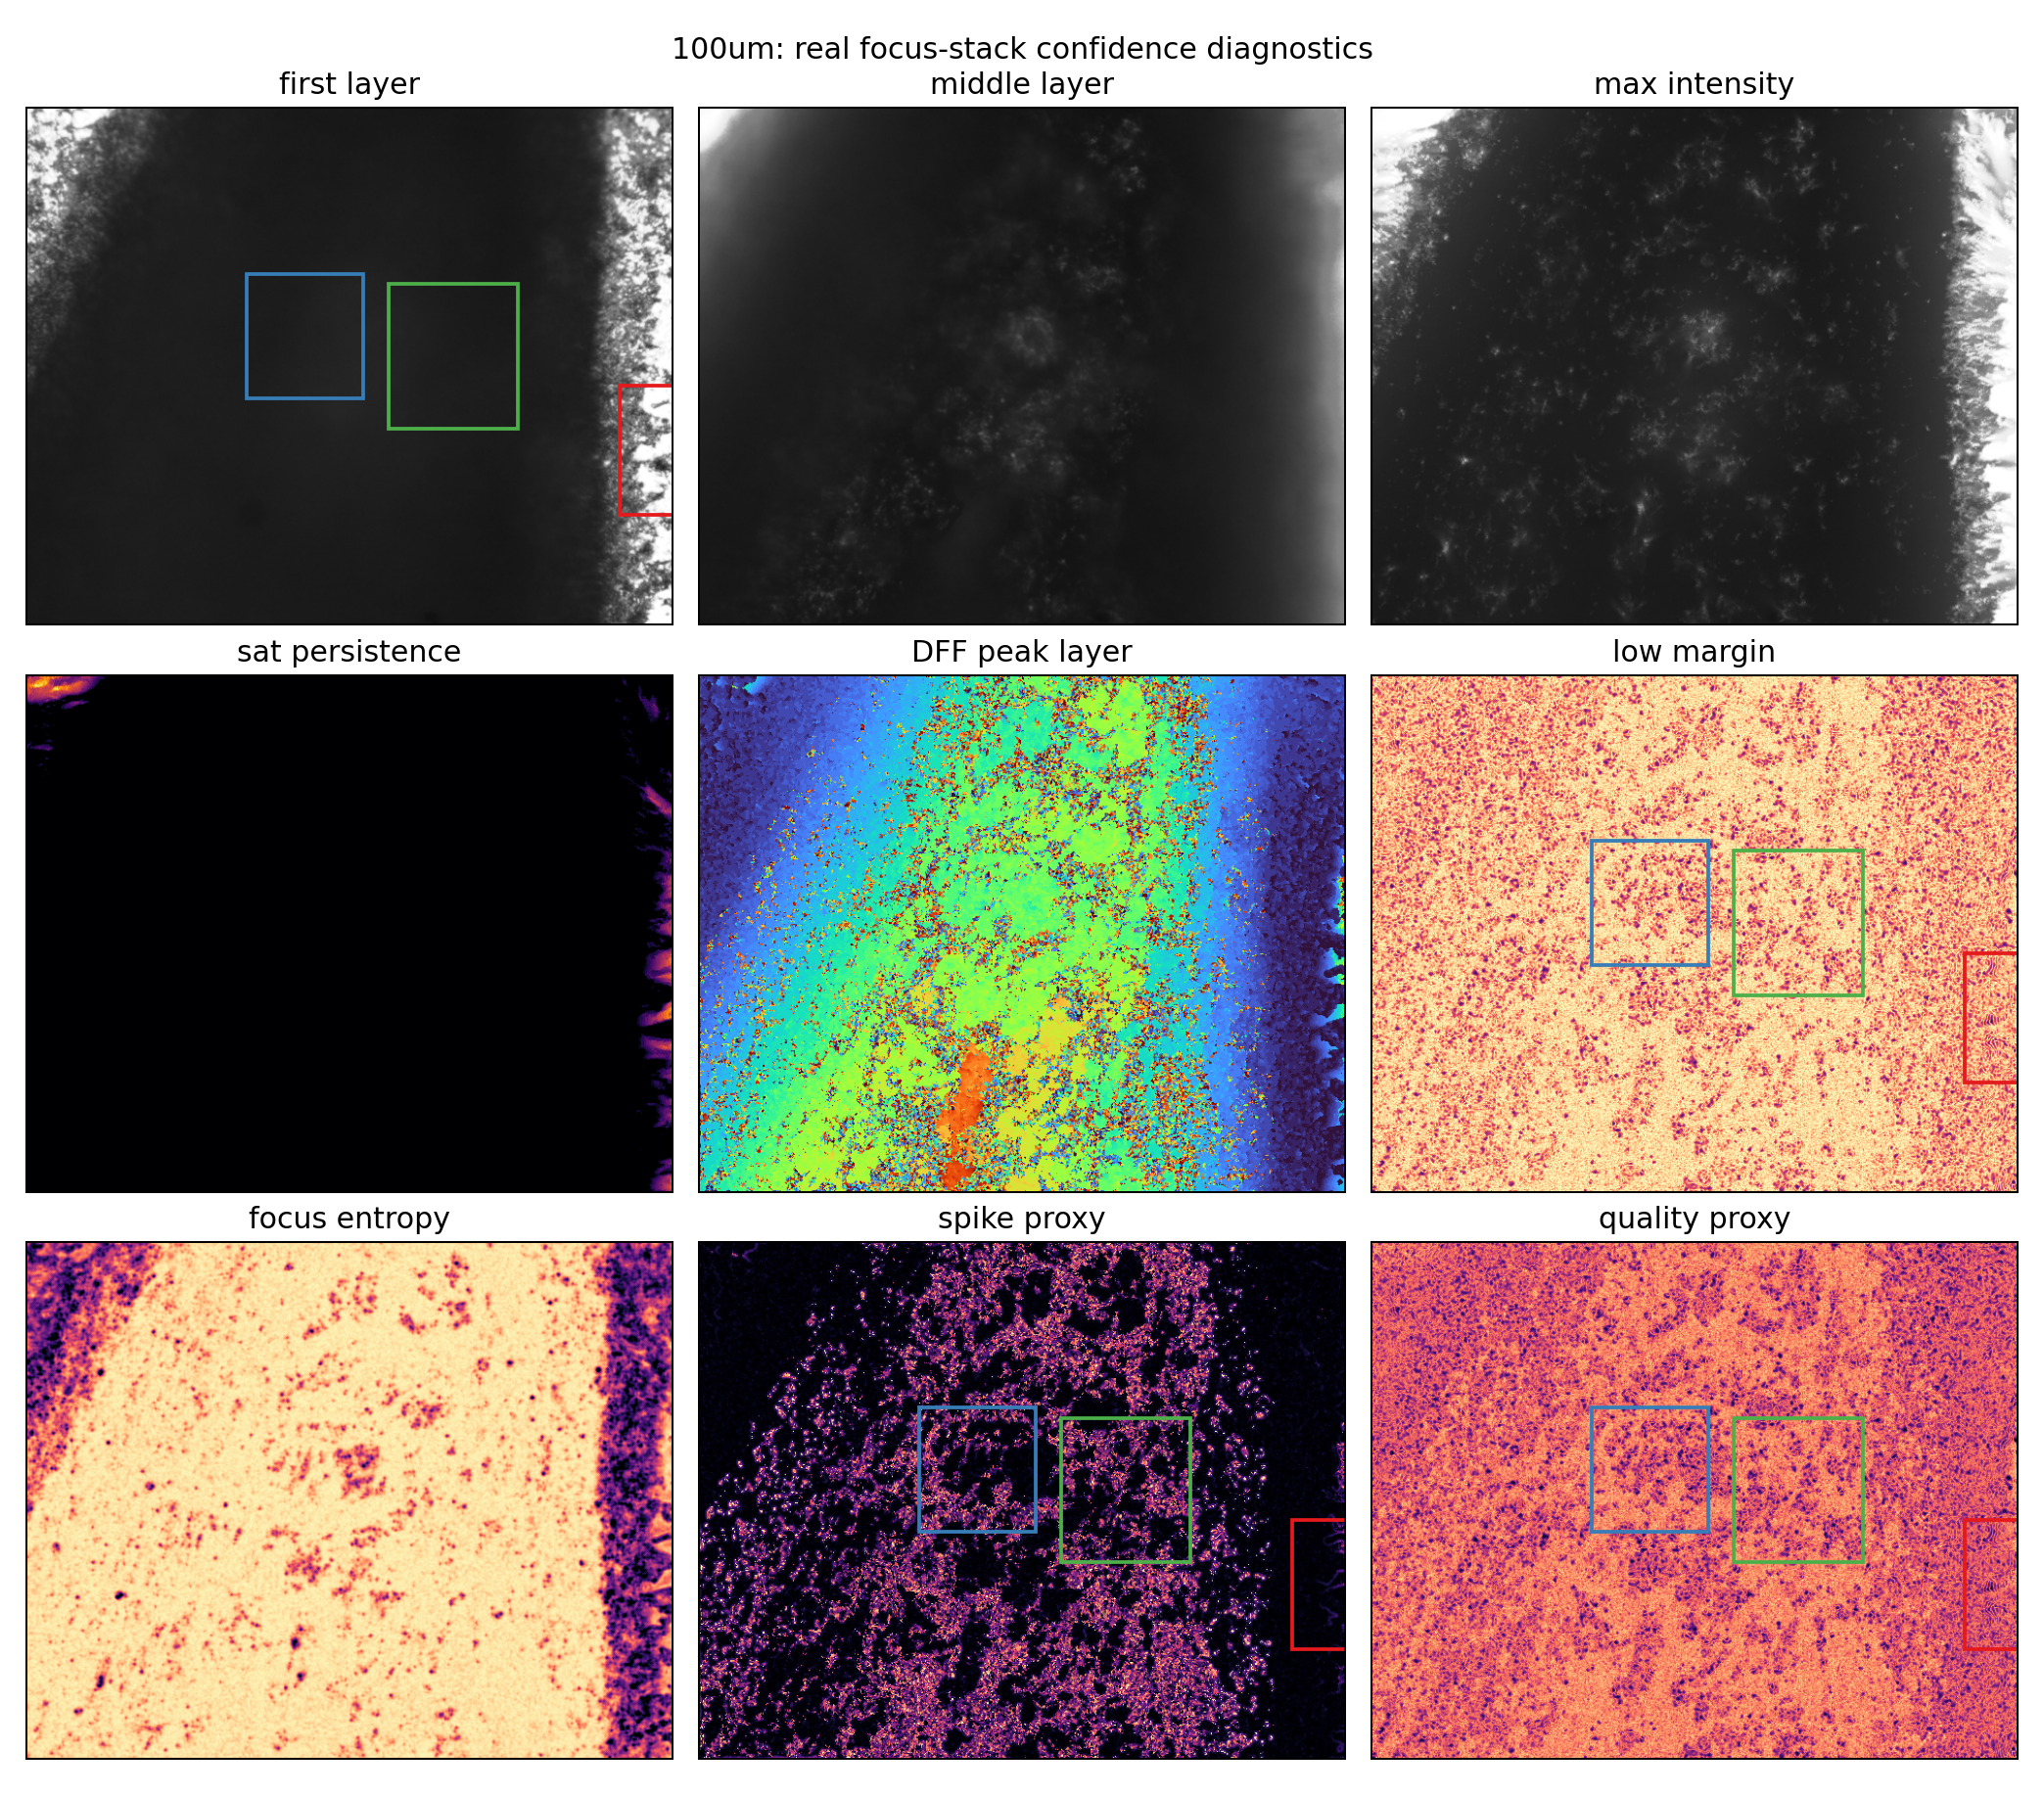
\includegraphics[width=\linewidth]{real_confidence_probe/钥匙纹路100um_real_confidence_maps.png}
\caption{Real focus-stack confidence maps for the 100um key-texture sample.}
\end{figure}

\begin{figure}[htbp]
\centering
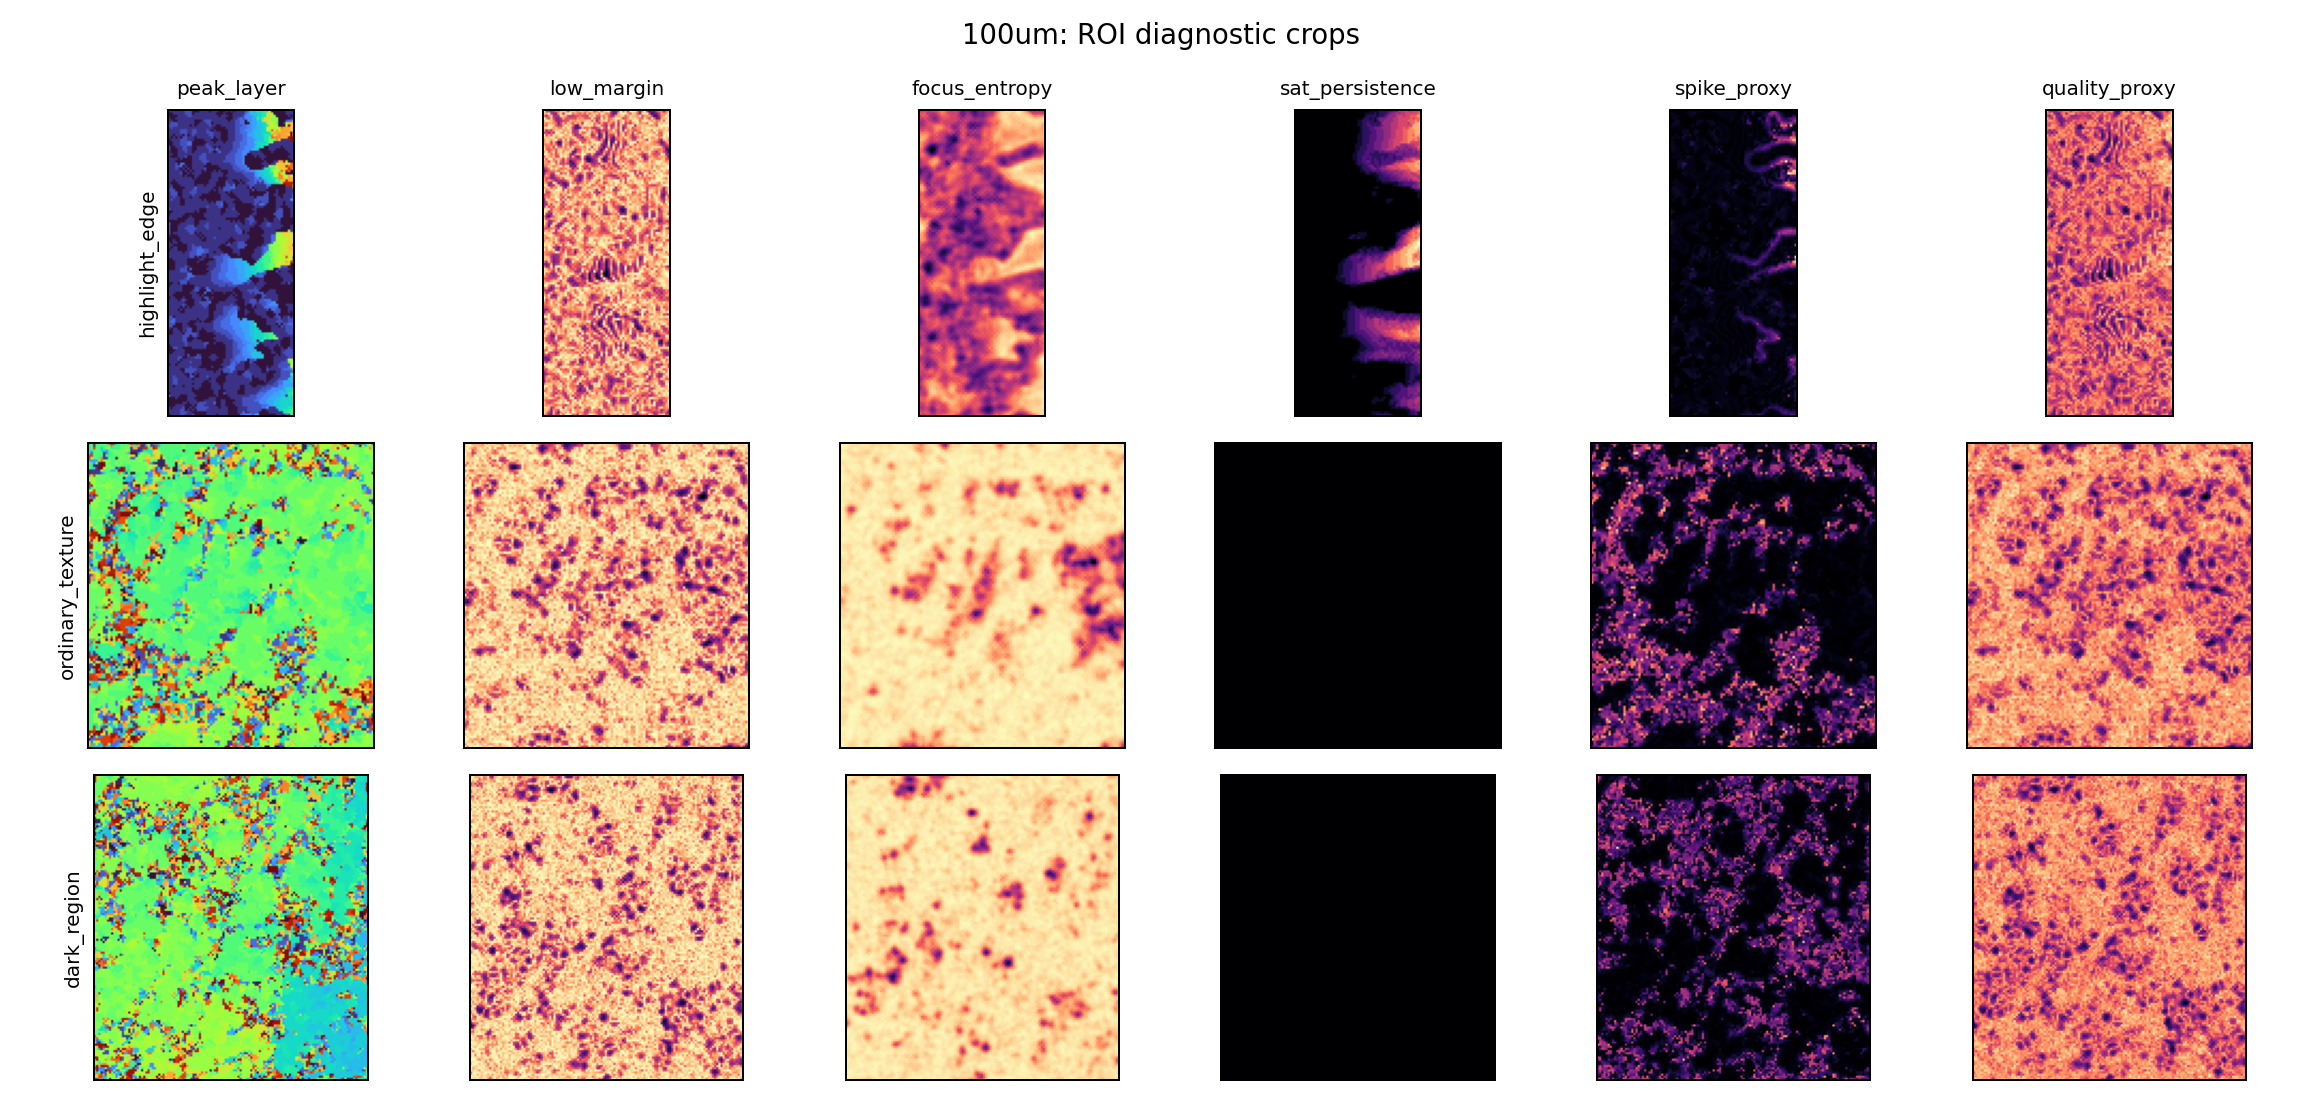
\includegraphics[width=\linewidth]{real_confidence_probe/钥匙纹路100um_real_roi_diagnostic_crops.png}
\caption{ROI crops for peak layer, confidence maps, saturation persistence, and spike proxy.}
\end{figure}

\section{Interpretation}

真实样本中存在两类不可靠性。第一类是早层高亮/过曝型不可靠性。The \texttt{highlight\_edge} ROI has a mean peak layer of 3.03 and non-zero saturation persistence, while the ordinary and dark ROIs have no persistent saturation and peak around layers 18--19. \texttt{sat\_persistence} and \texttt{bright\_persistence} identify saturation-related regions directly, with AUCs of 1.0000 and 0.9780 for saturation top10.

第二类是 DFF 层选择局部跳变型不可靠性。The ordinary and dark ROIs have higher spike-proxy means than the highlight ROI. The spike proxy is positively associated with \texttt{low\_margin}, \texttt{focus\_entropy}, and \texttt{low\_peak\_strength}. In particular, \texttt{low\_margin} reaches an AUC of 0.7293 for spike top10, while the combined \texttt{quality\_proxy} reaches 0.9289.

This partially supports the synthetic conclusion: focus confidence maps are useful no-reference indicators of DFF instability in real stacks. However, real data also shows that glare saturation and focus instability should be separated rather than collapsed into a single failure mask.

\section{Method Implication}

The real-stack quality prior can be written as:

\begin{equation}
Q_{\mathrm{real}}(x) =
\alpha (1 - M_{\mathrm{focus}}(x))
+ \beta H_{\mathrm{focus}}(x)
+ \gamma (1 - S_{\mathrm{peak}}(x))
+ \eta P_{\mathrm{sat}}(x),
\end{equation}

where the first three terms describe focus-response instability and $P_{\mathrm{sat}}$ describes glare or saturation persistence. In synthetic data, the weights can be calibrated with ground-truth height errors. In real stacks, the same quantity should be used as a visualization and diagnostic map, not as an error label.

\section{Paper-Ready Statement}

On the real focus stack of the 100um key-texture sample, we compute no-reference quality maps to examine whether the synthetic confidence prior corresponds to real focus-stack instability. The highlight-edge ROI has a mean DFF peak layer of 3.03 and non-zero saturation persistence, whereas the ordinary-texture and dark-region ROIs mainly peak around layers 18--19 with no persistent saturation. In contrast, local peak-layer discontinuities are more pronounced in the ordinary and dark regions. The spike proxy is positively associated with low margin, focus entropy, and low peak strength; the low-margin score achieves an AUC of 0.7293 for identifying the top 10\% spike-proxy pixels, while the combined quality proxy reaches 0.9289. These observations suggest two different types of unreliable regions in real stacks: early-layer glare/saturation artifacts and focus-response instability. Since real height ground truth is unavailable, these results are used as no-reference diagnostic evidence rather than absolute error measurements.

\section{Limitations}

This analysis does not use real height ground truth or strict inter-layer registration. Therefore, spike proxy should be interpreted as local discontinuity in the selected DFF layer, not as true height error. Saturation persistence indicates brightness abnormality, but it does not necessarily imply unrecoverable geometry. Future work should combine these proxies with real GT, WLI, confocal data, or carefully annotated ROIs.

\end{document}
